%%% Hlavní soubor. Zde se definují základní parametry a odkazuje se na ostatní části. %%%

%% Verze pro jednostranný tisk:
% Okraje: levý 40mm, pravý 25mm, horní a dolní 25mm
% (ale pozor, LaTeX si sám přidává 1in)
\documentclass[12pt,a4paper]{report}
\setlength\textwidth{145mm}
\setlength\textheight{247mm}
\setlength\oddsidemargin{15mm}
\setlength\evensidemargin{15mm}
\setlength\topmargin{0mm}
\setlength\headsep{0mm}
\setlength\headheight{0mm}
% \openright zařídí, aby následující text začínal na pravé straně knihy
\let\openright=\clearpage

%% Pokud tiskneme oboustranně:
% \documentclass[12pt,a4paper,twoside,openright]{report}
% \setlength\textwidth{145mm}
% \setlength\textheight{247mm}
% \setlength\oddsidemargin{14.2mm}
% \setlength\evensidemargin{0mm}
% \setlength\topmargin{0mm}
% \setlength\headsep{0mm}
% \setlength\headheight{0mm}
% \let\openright=\cleardoublepage

%% Vytváříme PDF/A-2u
\usepackage[a-2u]{pdfx}

%% Přepneme na českou sazbu a fonty Latin Modern
\usepackage[czech]{babel}
\usepackage{lmodern}
\usepackage[T1]{fontenc}
\usepackage{textcomp}

%% Použité kódování znaků: obvykle latin2, cp1250 nebo utf8:
\usepackage[utf8]{inputenc}

%%% Další užitečné balíčky (jsou součástí běžných distribucí LaTeXu)
\usepackage{amsmath}        % rozšíření pro sazbu matematiky
\usepackage{amsfonts}       % matematické fonty
\usepackage{amsthm}         % sazba vět, definic apod.
\usepackage{bbding}         % balíček s nejrůznějšími symboly
			    % (čtverečky, hvězdičky, tužtičky, nůžtičky, ...)
\usepackage{bm}             % tučné symboly (příkaz \bm)
\usepackage{graphicx}       % vkládání obrázků
\usepackage{fancyvrb}       % vylepšené prostředí pro strojové písmo
\usepackage{indentfirst}    % zavede odsazení 1. odstavce kapitoly
\usepackage{natbib}         % zajištuje možnost odkazovat na literaturu
			    % stylem AUTOR (ROK), resp. AUTOR [ČÍSLO]
\usepackage[nottoc]{tocbibind} % zajistí přidání seznamu literatury,
                            % obrázků a tabulek do obsahu
\usepackage{icomma}         % inteligetní čárka v matematickém módu
\usepackage{dcolumn}        % lepší zarovnání sloupců v tabulkách
\usepackage{booktabs}       % lepší vodorovné linky v tabulkách
\usepackage{paralist}       % lepší enumerate a itemize
\usepackage[usenames]{xcolor}  % barevná sazba
\usepackage{listings}

%% Moje package
\usepackage{lipsum}                     % Dummytext
\usepackage{xargs}                      % Use more than one optional parameter in a new commands
% 
\usepackage[colorinlistoftodos,prependcaption,textsize=tiny]{todonotes}

%%% Údaje o práci

% Název práce v jazyce práce (přesně podle zadání)
\def\NazevPrace{Evoluční algoritmy pro řízení heterogenních robotických swarmů}

% Název práce v angličtině
\def\NazevPraceEN{Evolutionary Algorithms for the Control of Heterogeneous Robotic Swarms}

% Jméno autora
\def\AutorPrace{Tomáš Karella}

% Rok odevzdání
\def\RokOdevzdani{2017}

% Název katedry nebo ústavu, kde byla práce oficiálně zadána
% (dle Organizační struktury MFF UK, případně plný název pracoviště mimo MFF)
\def\Katedra{Katedra teoretické informatiky a matematické logiky}
\def\KatedraEN{Department of Theoretical Computer Science and Mathematical Logic at Faculty of Mathematics and Physics}

% Jedná se o katedru (department) nebo o ústav (institute)?
\def\TypPracoviste{Katedra}
\def\TypPracovisteEN{Department}

% Vedoucí práce: Jméno a příjmení s~tituly
\def\Vedouci{Mgr. Martin Pilát, Ph.D.}

% Pracoviště vedoucího (opět dle Organizační struktury MFF)
\def\KatedraVedouciho{Katedra teoretické informatiky a matematické logiky}
\def\KatedraVedoucihoEN{Department of Theoretical Computer Science and Mathematical Logic}

% Studijní program a obor
\def\StudijniProgram{Informatika}
\def\StudijniObor{Programování a Softwarové Systémy}

% Nepovinné poděkování (vedoucímu práce, konzultantovi, tomu, kdo
% zapůjčil software, literaturu apod.)
\def\Podekovani{%
Poděkování.
}

% Abstrakt (doporučený rozsah cca 80-200 slov; nejedná se o zadání práce)
\def\Abstrakt{%
Abstrakt.
}
\def\AbstraktEN{%
Abstract.
}

% 3 až 5 klíčových slov (doporučeno), každé uzavřeno ve složených závorkách
\def\KlicovaSlova{%
{klíčová} {slova}
}
\def\KlicovaSlovaEN{%
{key} {words}
}

%% Balíček hyperref, kterým jdou vyrábět klikací odkazy v PDF,
%% ale hlavně ho používáme k uložení metadat do PDF (včetně obsahu).
%% Většinu nastavítek přednastaví balíček pdfx.
\hypersetup{unicode}
\hypersetup{breaklinks=true}

%% Definice různých užitečných maker (viz popis uvnitř souboru)
%%% Tento soubor obsahuje definice různých užitečných maker a prostředí %%%
%%% Další makra připisujte sem, ať nepřekáží v ostatních souborech.     %%%

%%% Drobné úpravy stylu

% Tato makra přesvědčují mírně ošklivým trikem LaTeX, aby hlavičky kapitol
% sázel příčetněji a nevynechával nad nimi spoustu místa. Směle ignorujte.
\makeatletter
\def\@makechapterhead#1{
  {\parindent \z@ \raggedright \normalfont
   \Huge\bfseries \thechapter. #1
   \par\nobreak
   \vskip 20\p@
}}
\def\@makeschapterhead#1{
  {\parindent \z@ \raggedright \normalfont
   \Huge\bfseries #1
   \par\nobreak
   \vskip 20\p@
}}
\makeatother

% Toto makro definuje kapitolu, která není očíslovaná, ale je uvedena v obsahu.
\def\chapwithtoc#1{
\chapter*{#1}
\addcontentsline{toc}{chapter}{#1}
}

% Trochu volnější nastavení dělení slov, než je default.
\lefthyphenmin=2
\righthyphenmin=2

% Zapne černé "slimáky" na koncích řádků, které přetekly, abychom si
% jich lépe všimli.
\overfullrule=1mm

%%% Makra pro definice, věty, tvrzení, příklady, ... (vyžaduje baliček amsthm)

\theoremstyle{plain}
\newtheorem{veta}{Věta}
\newtheorem{lemma}[veta]{Lemma}
\newtheorem{tvrz}[veta]{Tvrzení}

\theoremstyle{plain}
\newtheorem{definice}{Definice}

\theoremstyle{remark}
\newtheorem*{dusl}{Důsledek}
\newtheorem*{pozn}{Poznámka}
\newtheorem*{prikl}{Příklad}

%%% Prostředí pro důkazy

\newenvironment{dukaz}{
  \par\medskip\noindent
  \textit{Důkaz}.
}{
\newline
\rightline{$\square$}  % nebo \SquareCastShadowBottomRight z balíčku bbding
}

%%% Prostředí pro sazbu kódu, případně vstupu/výstupu počítačových
%%% programů. (Vyžaduje balíček fancyvrb -- fancy verbatim.)

\DefineVerbatimEnvironment{code}{Verbatim}{fontsize=\small, frame=single}

%%% Prostor reálných, resp. přirozených čísel
\newcommand{\R}{\mathbb{R}}
\newcommand{\N}{\mathbb{N}}

%%% Užitečné operátory pro statistiku a pravděpodobnost
\DeclareMathOperator{\pr}{\textsf{P}}
\DeclareMathOperator{\E}{\textsf{E}\,}
\DeclareMathOperator{\var}{\textrm{var}}
\DeclareMathOperator{\sd}{\textrm{sd}}

%%% Příkaz pro transpozici vektoru/matice
\newcommand{\T}[1]{#1^\top}

%%% Vychytávky pro matematiku
\newcommand{\goto}{\rightarrow}
\newcommand{\gotop}{\stackrel{P}{\longrightarrow}}
\newcommand{\maon}[1]{o(n^{#1})}
\newcommand{\abs}[1]{\left|{#1}\right|}
\newcommand{\dint}{\int_0^\tau\!\!\int_0^\tau}
\newcommand{\isqr}[1]{\frac{1}{\sqrt{#1}}}

%%% Vychytávky pro tabulky
\newcommand{\pulrad}[1]{\raisebox{1.5ex}[0pt]{#1}}
\newcommand{\mc}[1]{\multicolumn{1}{c}{#1}}


%% Titulní strana a různé povinné informační strany
\begin{document}
%%% Titulní strana práce a další povinné informační strany

%%% Titulní strana práce

\pagestyle{empty}
\hypersetup{pageanchor=false}

\begin{center}

\centerline{\mbox{
\includegraphics[width=166mm]{../img/logo-cs.pdf}}}

\vspace{-8mm}
\vfill

{\bf\Large BAKALÁŘSKÁ PRÁCE}

\vfill

{\LARGE\AutorPrace}

\vspace{15mm}

{\LARGE\bfseries\NazevPrace}

\vfill

\Katedra

\vfill

\begin{tabular}{rl}

Vedoucí bakalářské práce: & \Vedouci \\
\noalign{\vspace{2mm}}
Studijní program: & \StudijniProgram \\
\noalign{\vspace{2mm}}
Studijní obor: & \StudijniObor \\
\end{tabular}

\vfill

% Zde doplňte rok
Praha \RokOdevzdani

\end{center}

\newpage

%%% Následuje vevázaný list -- kopie podepsaného "Zadání bakalářské práce".
%%% Toto zadání NENÍ součástí elektronické verze práce, nescanovat.

%%% Strana s čestným prohlášením k bakalářské práci

\openright
\hypersetup{pageanchor=true}
\pagestyle{plain}
\pagenumbering{roman}
\vglue 0pt plus 1fill

\noindent
Prohlašuji, že jsem tuto bakalářskou práci vypracoval(a) samostatně a výhradně
s~použitím citovaných pramenů, literatury a dalších odborných zdrojů.

\medskip\noindent
Beru na~vědomí, že se na moji práci vztahují práva a povinnosti vyplývající
ze zákona č. 121/2000 Sb., autorského zákona v~platném znění, zejména skutečnost,
že Univerzita Karlova má právo na~uzavření licenční smlouvy o~užití této
práce jako školního díla podle §60 odst. 1 autorského zákona.

\vspace{10mm}

\hbox{\hbox to 0.5\hsize{%
V ........ dne ............
\hss}\hbox to 0.5\hsize{%
Podpis autora
\hss}}

\vspace{20mm}
\newpage

%%% Poděkování

\openright

\noindent
\Podekovani

\newpage

%%% Povinná informační strana bakalářské práce

\openright

\vbox to 0.5\vsize{
\setlength\parindent{0mm}
\setlength\parskip{5mm}

Název práce:
\NazevPrace

Autor:
\AutorPrace

\TypPracoviste:
\Katedra

Vedoucí bakalářské práce:
\Vedouci, \KatedraVedouciho

Abstrakt:
\Abstrakt

Klíčová slova:
\KlicovaSlova

\vss}\nobreak\vbox to 0.49\vsize{
\setlength\parindent{0mm}
\setlength\parskip{5mm}

Title:
\NazevPraceEN

Author:
\AutorPrace

\TypPracovisteEN:
\KatedraEN

Supervisor:
\Vedouci, \KatedraVedoucihoEN

Abstract:
\AbstraktEN

Keywords:
\KlicovaSlovaEN

\vss}

\newpage

\openright
\pagestyle{plain}
\pagenumbering{arabic}
\setcounter{page}{1}


%%% Strana s automaticky generovaným obsahem bakalářské práce

\tableofcontents

%%% Jednotlivé kapitoly práce jsou pro přehlednost uloženy v samostatných souborech
\chapter*{Úvod}
\addcontentsline{toc}{chapter}{Úvod}

\title{Úvod}
Využití robotických hejn (robotic swarms) patří mezi rentabilní metody pro řešení složitějších úkolů. Existuje řada studií potvrzujících, že velký počet jednoduchých robotů dokáže plně nahradit komplexnější jedince. Dostatečná velikost hejna umožní řešení úloh, které by jednotlivec z hejna provést nesvedl. Navíc robotické hejno přináší několik výhod díky kvantitě jsou odolnější proti poškození i po zničení některých z nich zbytek robotů pokračuje v plnění cílů. Dále výroba jednodušších robotů vychází levněji než komplexních jedinců, což přináší nezanedbatelnou výhodu pro práci v nebezpečném prostředí. Hejno také může pokrývat vícero různých úkolů než specializovaný robot, který bude při plnění úkolů, lišících se od typu úloh zamýšlených při konstrukci, mnohem více nemotorný a nejspíše pomalejší. Hejno pokryje větší plochu při plnění úkolů. 
\par
Existuje mnoho aplikací robotických hejn, vetšinou se používají v úlohách týkajících se průzkumu a mapování prostředí, hledání nejkratších cest, nasazení v nebezpečných místech. Jako příklad můžeme uvést asistenci záchranným složkám při požáru \citep{fireRobots}. Mnoho projektů zabývající se řízením robotického hejna se inspiruje přírodou, používá se analogie s chováním mravenců a jiného hmyzu \citep{PheroRobot}. Objevují se i hardwarové implementace chování hejn, zmiňme projekty Swarm-bots \citep{swarmBots}, Colias \citep{Colias}  
\par 
Elementárnost senzorů i efektorů jednotlivých robotů vybízí k použití evolučních algoritmů, jelikož prostor řešení je rozlehlý a plnění cílů lze vhodně ohodnotit. Vzniklo několik vědeckých prací popisující problematiku tohoto tématu \citep{ENovel} \citep{geneticSwarm}.
\section*{Cíl práce}
Všechny zmíněné práce používají pro tvorbu řídicích programů evoluční algoritmy (EA) a pracují pouze s homogenními hejny. Cílem této práce je vyzkoušet využití EA na generování chování hejna heterogenních robotů, tedy skupiny agentů, ve které se objevuje několik druhů jedinců a společně plní daný úkol. V rámci práce byl vytvořen program pro simulaci různých scénářů. Pro otestování jejich úspěšnosti v rámci EA, byly zvoleny 3 odlišné scénáře, ve kterých se objevují 2-3 druhy robotů.
\section*{Struktura práce}
Rozdělení práce je následující. První kapitola je věnována obecnému úvodu do tématiky evolučních algoritmů, kde se podrobněji věnuji evolučním strategiím a diferenciální evoluci, protože oba tyto postupy implementuji v programu pro řešení scénářů. Druhá kapitola se zabývá představením robotického hejna, základním principům a několika konkrétnějším aplikacím. Ve třetí kapitole je nastíněno fungování simulátoru, přiložené dokumentace obsahuje podrobnější informace o implementaci simulátoru. Všechny provedené experimenty se všemi detaily obsahuje čtvrtá kapitola.
\chapter{Evoluční algoritmy}
\section{Historie}
Začněme pohledem do historie Evolučních algoritmů na základě knih \citep{MitchellBook} a \citep{eibenIntro}. Darwinova myšlenka evoluce lákala vědce už před průlomem počítačů, Turing vyslovil myšlenku \textit{genetického a evolučního vyhledávání} už v roce 1948. V 50. a 60. letech nezávisle na sobě vznikají 4 hlavní teorie nesoucí podobnou myšlenku. Společným základem všech teorií byla evoluce populace kandidátů na řešení daného problému a jejich následná úprava způsoby hromadně nazývány jako genetické operátory, například mutace genů, přirozená selekce úspěšnějších řešení. \par 
Rechenberg a Schwefell (1965, 1973) představuje \textit{Evoluční strategie}, metoda optimalizující parametry v reálných číslech, jejich použití pro letadlová křídla. Fogel, Owens, Walsh zveřejňují \textit{evolutionary programming}(evoluční programování), technika využívající k reprezentaci kandidátů konečný automat(s konečným počtem stavů), který je vyvíjen mutací přechodů mezi stavy a následnou selekcí. \textit{Genetické algoritmy} vynalezl Holand v 60. letech a následně se svými studenty a kolegy z Michiganské Univerzity implementoval, oproti ES a EP nebylo hlavním cílem formovat algoritmus pro řešení konkrétních problémů, ale přenos obecného mechanismu evoluce jako metody aplikovatelné v informatickém světě. Princip GA spočívá v transformaci populace chromozonů(př. vektor 1 a 0) v novou populaci pomocí genetických operátorů křížení, mutací a inverze. V 1975 v knize \textit{Adaptation in Natural and  Artificial Systems} \citep{HolandBook} definoval genetický algoritmus jako abstrakci biologické evoluce spolu s teoretickým základem jejich používání. Ovšem někteří vědci používají pojem GA i ve významech hodně vzdálených původní Holandově definici. K sjednocení jednotlivých přístupů přispěl v 90. letehc Koza, dále jsou všechny zahrnuty jako oblasti \textit{Evolučních algoritmů}. Dnes existuje řada konferencí a odborných časopisů sdružující pracovníky zabývající se touto oblastí. Zmiňme ty větší z nich, co se týče konferencí: 
\href{http://gecco-2017.sigevo.org/index.html/HomePage}{GECCO}, \href{http://www.ppsn2016.org/conference}{PPSN}, 
\href{http://www.cec2017.org/}{CEC}, 
\href{http://www.evostar.org/2018/}{EVOSTAR}, 
časopisy: 
\href{http://www.mitpressjournals.org/loi/evco}{Evolutionary Computation}, 
\href{http://ieeexplore.ieee.org/xpl/RecentIssue.jsp?reload=true&punumber=4235}{IEEE Transactions on Evolutionary Computation}, 
\href{http://www.springer.com/computer/ai/journal/10710}{Genetic Programming and Evolvable Machines},
\href{https://www.journals.elsevier.com/swarm-and-evolutionary-computation/}{Swarm and Evolutionary Computation}
\section{Obecný evoluční algoritmus)
Popišme si základní myšlenku všech evolučních algoritmů. Jedná se o stochastické prohledávací algoritmy, které jsou inspirované přírodou. Slouží k prohledávání prostoru řešení daného řešeného problému. 
\subsection{Jedinec}
Jedinec reprezentuje kandidáta na řešení problému. Může být reprezentován různými způsoby, např. v kontextu l-bitové vektory(GA), konečné automaty(EP), reálné vektory(ES). 
\subsection{Populace}
Populace označuje množinu jedinců.
\subsection{Generace}
Generace je populaci jednotlivého kroku EA.
\subsection{Fitness}
Fitness je funkce, která každému jedinci přiřadí reálné číslo, slouží k ohodnocení úspěšnosti kandidáta v kotextu řešeného problému. Pomocí EA se snažíme maximalizovat fitness v rámci další generace. Cíle EA je tedy nalézt jedince s nejvyšší fitness. 
\subsection{Kritérium ukončení}
Kritérium ukončení určuje koncovou podmínky pro ukončení prohledávání prostoru řešení. Většinou se jedná o počet generací, časový limit nebo dosáhnutí určité hodnoty fitness.  
\subsection{Základ EA}
Nejdříve se náhodně vygenerujeme inicializační populaci(P(0)), ohodnotíme jedince pomocí fitness funkce. Dokud není splněno koncové kritérium opakujeme následujíci algoritmus z P(t) vytvářej P(t+1). \par
\begin{itemize}
    \item Výběr z rodičů 
    \item Rekombinace jedinců a jejich následná mutace, co odpovídá vzniku nových jedinců
    \item Ohodnocení nově vzniklých jedinců
    \item Enviromentální selekce ta vybere P(t+1) z P(t) a nově vzniklých jedinců
\end{itemize}

%%% Druhá kapitola

\chapter{Robotický swarm}
Myšlenka robotického swarmu pochází podobně jako u genetických algoritmů z inspirace matkou Přírodou. Podle souhrnu \citep{swarmRobotic} popíši základní myšlenku RS. Pro robotický swarm se také používá výraz rojová robotika či robotický roj, v angličtině je známý pod pojmem swarm robotics. 
\section*{Základní vlastnosti}
Motivací pro použití RS může být chování živočichů na Zemi. Zaměříme se na skupiny živočichů jako jsou mravenci, včely, ryby dokonce i některé savce. Pokud bychom vložili do prostředí jednotlivce z některé ze zmíněných skupin, nebude schopen konkurovat nepřátelskému prostředí a nejspíše příliš dlouho nepřežije. Na druhou stranu, když budeme uvažovat celé společenství, tak se nám ze slabého jedince stane velmi adaptivní, odolný a rychle se vyvíjející roj. Podobnému účinku bychom se chtěli přiblížit v RS. Pro relativně jednoduchého robota, který není schopen plnit obtížný úkol, se pokusíme použít vícero robotů stejného typu, kteří společně zadaný úkol vyřeší. Navíc chceme těžit ze všech výhod hejna. \par. 
\par
Jako nejčastější výhody RS oproti jednomu robotovi se nejčastěji uvádějí:
    \begin{enumerate}
        \item Paralelita - Díky malé ceně jedince, si můžeme dovolit velkou populaci jedinců. Malou cenou jedince v ES myslíme, že se jedná o jednoduchého robota s nízkou pořizovací cenou. V kontextu živočichů můžeme uvažovat množství energie, jídla pro tvorbu takového jedince. Velká populace nám umožňuje řešit vícero úkolů naráz, také na velké ploše. Zvláště pro vyhledávací úkoly ušetříme nemalé množství času. 
        \item Škálovnatelnost - Změna velikosti populace hejna neovlivní chování ostatních jedinců. Samozřejmě plnění úkolu bude rychlejší či pomalejší, ale původní hejno bude stále plnit původní úkol. Tím pádem můžeme celkem snadno upravovat velikost populace bez větší obtíží. V přírodě můžeme pozorovat, že smrt  jednotlivých mravenců-dělníků znatelně neovlivní práci celého mraveniště. Nově narození mravenci se mohou vydat do práce, zatímco zbytek mraveniště nemění činnost. 
        \item Houževnatost - Související se škálovatelností, jen v tomto případě máme na mysli necílenou změnu populace. Jako v předchozím příkladu, u smrti mravenců, část robotů ES může selhat z rozličných důvodů, zbytek hejna však bude pokračovat k cíli, i když ve výsledku jim bude jeho dosáhnutí trvat o něco déle. To se nám může vyplatit v nebezpečných prostředích. 
        \item Ekonomické výhody - Cena návrhu a konstrukce jednoduchých hejn robotů vyjde většinou levněji než jeden specializovaný robot schopný uspokojit stejné požadavky. V dnešním světě vychází výroba ve velkém množství mnohem levněji než tvorba jednoho drahého konkrétního robota.
        \item Úspora energie - Díky menší velikosti a složitosti jednotlivých robotů vyžadují mnohem menší množství energie. To má za důsledek, že si u nich můžeme dovolit energetickou rezervu na delší čas. Navíc když je pořizovací cena jednoho robota menší než náklady na dobití, můžeme díky škálovatelnosti pouze připojit nové roboty, což u drahého robota jde málokdy. 
        \item Autonomie a decentralizace - V kontextu RS musí každý jedinec hejna jednat autonomně, jedinci nejsou řízeni žádnou autoritou. Takže umí pracovat i při ztrátě komunikace. Opět se vychází z chování živých organismů. Pokud se chovají jedinci hejna dostatečně kooperativně, mohou pracovat bez centrálního řízení, důsledkem toho se stává celé hejno ještě flexibilnější a odolnější, hlavně v prostředích s omezenou komunikací. Navíc hejno mnohem rychleji reaguje na změny. 
    \end{enumerate}
\par 
Mimo RS existuje i řada jiných přístupů, které se inspirovaly životem hejn v přírodě. Občas jsou zaměňovány za RS, nejčastěji se jedná o multi-agentní systémy a senzorové sítě (sensor networks). V následující tabulce jsou popsány jejich nejklíčovější vlastnosti. \par
\begin{center}
    \begin{table}[h] \resizebox{\textwidth}{!}{%
    \begin{tabular}{l l l l l @{\hspace{1.5cm}}D{.}{,}{3.2}D{.}{,}{1.2}D{.}{,}{2.3}}
            \toprule
             & \textbf{Robotická hejna} & \textbf{Multi-robotické systémy} & \textbf{Senzorové sítě} & \textbf{Multi-agentní systémy} \\
            \textbf{Velikost populace }& Variabilní ve velkém rozsahu & Malá & Fixní & V malém rozsahu \\
            \textbf{Řízení} & decentralizované a autonomní & centralizované & centralizované & centralizované \\
            \textbf{Odlišnosti} & většinou homogenní & většinou heterogenní & homogenní & homogenní nebo heterogenní \\
            \textbf{Flexibilita} & vysoká & nízká & nízká & střední \\
            \textbf{Škálovnatelnost} & vysoká & nízká & střední & střední \\
            \textbf{Prostředí} & neznámé & známé nebo neznámé & známé & známé\\
            \textbf{Pohyblivost} & ano & ano & ne & vyjímečně\\
            \hline 
    \end{tabular}}
	\caption{Porovnání systémů s více agenty}
    \end{table}
    \end{center}
    Jednotlivé systémy s více agenty se také liší svojí aplikací. Robotická hejna se nejčastěji používají ve vojenských, nebezpečných úkolech a také pro řešení ekologických katastrof. Multi-robotické systémy potkáváme v transportních, skenovacích úkolech, dále pro řízení robotických fotbalových hráčů. Oproti tomu nejčetnější využití senzorových sítí zasahuje do medicínské oblasti, ochrany životního prostředí. Multi-agentní systémy zase nejvíce zasahují do řízení síťových zdrojů a distribuovaného řízení. 
\section{Použití}
Existuje několik vědeckých prací, které studují a navrhují použití RS v reálném nasazení. 
\par 
Některé jsem zmínil už v úvodu této práce, jako například hasičům asistující roboty \citep{fireRobots}.  Zde si robotické hejno klade za cíl usnadnit a podpořit navigaci lidem v nebezpečném prostředí. Jejich využití je ilustrováno záchranou misí ve velkém skladišti. Hasiči mají díky kouři velmi omezenou viditelnost. Tím pádem se lokalizace přeživších, epicenter požárů a další důležitých bodů stává obtížným a zdraví ohrožujícím úkolem. Nezřídka se stává, že zasahující hasič zahyne, protože se v hustém dýmu v objektu ztratil. Robotické hejno tedy může prozkoumat celý prostor před vlastním zásahem. Při zásahu ještě asistovat hasičům při orientaci v prostoru. 
\par
Robotická hejna se také ukázala jako užitečná u ekologický pohrom. Španělští vědci testovali jejich použití při úniku ropy \citep{oilSwarm}, či při hledání centra radiace \citep{radiationSwarm}. 
\par 
V prvně zmíněném příkladu autoři mapovali znečištění mořské vody. Dokonce při plavbách bez defektů se do moře uvolňuje palivo, ropa a další nebezpečné látky. Očekává se, že s rostoucí námořní dopravou se rozrostou tyto lokální znečištění ve vážnou hrozbu. Aktuální systémy monitorující znečištění při katastrofách tankerů jsou pro toto využití příliš drahé. Autoři proto navrhují použití hejna dronů, které bude dokumentovat velké vodní plochy a bude schopno odhalovat případné nebezpečí a větší koncentrace cizích látek. Dokonce budou moci na základě získaných informací sledovat znečisťovatele. 
\par
Po jaderné katastrofě se stává explorace zamořené oblasti  v podstatě nemožným úkolem pro lidské průzkumníky. Právě monitorování radiací postiženým územím se stala motivací pro práci \citep{radiationSwarm}. Ve zmiňované práci se autoři soustředí na porovnávání autonomních robotických hejn a RS komunikujících s člověkem. V rámci výsledků ukazují, výhody použití robotického hejna pro hledání centra radiace a také že RS interagující s lidmi dosahují lepších výsledků.
\par
Několik prací nezůstalo pouze u simulací a také využívali RS u fyzických robotů. Hlavní motivací pro práci \citep{aquaticRobots} byl fakt, že většinou se řízení RS vytváří  a hlavně testuje pouze v uzavřeném a simulovaném prostředí. Tvůrci se rozhodli pro reálné použití na moři, kde nemohou prostředí jakkoli ovládat či kontrolovat. Snaží se tím ukázat, že i přes šumy a neočekávané situace, RS je stabilní a použitelné pro aplikaci ve skutečném světě. Celé hejno se skládalo z deseti robotů. Jednalo se o malé lodičky s délkou přibližně 60 cm a nízkou pořizovací cenou okolo 300 euro. Každý robot byl  vybaven GPS, WIFI, kompasem. Chování bylo připraveno pomocí evolučních algoritmů v simulaci, konkrétně autoři používají neuroevoluci NEAT, jejich simulace obsahovala 4 podúkoly: navádění, shlukování, rozptylování a monitorování prostředí. Poté bylo stvořené řízení ohodnoceno na vodní ploše. Prezentované výsledky vypadají velmi slibně, chování a úspěšnost řízení se velmi blíží mezi simulací a reálným nasazením. Také potvrzují přítomnost výhodných vlastností ze simulaci v reálném světě, jedná se o robustnost, flexibilitu, škálovatelnost. V neposlední řadě také úspěšnost skládání jednoduchých podúkolů do komplexního chování v rámci hejna, které řeší složitý hlavní cíl.  
\section{Řízení robotických swarmů}
Chování swarmů se řadí mezi velmi obtížné úkoly pro svět informatiky. Pro reprezentaci chování se využívá \textit{neuronových sítí}, které se optimalizují pomocí nastavování vah jednotlivých perceptronů, neboť se jedná o velký prostor vstupních informací ze senzorů a prostor pro interakci s prostředím je taktéž velmi rozsáhlý. Přímé prohledávání takto obřího prostoru nepřichází v úvahu, proto v poslední době získávají na oblibě evoluční algoritmy. Mezi nejvíce používané patří evoluční strategie, či genetické programování. \par 

\subsection*{Genetické programování a stromy chování}
V práci \uv{Evolving behaviour trees for Swarm robotics} \citep{Jones2018} se autoři zaměřují na využití genetického programování pro vytvoření chování robotického hejna. Pro řízení hejna navrhují vcelku zajímavé využití stromů chování (SC)(behaviour tree), které mají uplatnění především v herním průmyslu pro akce charakterů, které nejsou ovládány hráčem. Jako optimalizační algoritmus zvolili genetické programování. 
\par
Strom chování je strom, jehož listy interagují s prostředím, vnitřní vrcholy spojují tyto akce dohromady a tvoří rozhodovací a závislostní pravidla. Celý strom je vyhodnocován v pravidelných intervalech, v práci se značí jako \textit{tick}. Opírají se o článek \citep{shoulson2011parameterizing}, kde bylo ukázáno, že SC může plnohodnotně reprezentovat konečné automaty, dokonce i když budeme používat pravděpodobností konečné automaty. Jako jedince z hejna zvolili Kilobot, které byl představen Rubensteinen v \citep{Kilobots}. Kiloboti se pohybuji pomocí dvou vibračních motorů, komunikují přes infračervený kanál, v prostředí se orientují pomocí foto detektoru a signalizují pomocí LED diod s barevným spektrem. Tabulka \ref{tab02:behatree} ukazuje, jak byla zjednodušena komunikace s efektory robota a nad nimi optimalizováno SC. 
\par
\begin{table}[h]\resizebox{\textwidth}{!}{%
		\begin{tabular}{l l l l l @{\hspace{1.5cm}}D{.}{,}{3.2}D{.}{,}{1.2}D{.}{,}{2.3}}
        \toprule
        Efektor/Senzor & Read or Write & Popis \\
        \midrule
        motor & W & vypnut, vřed, vlevo, vpravo \\
        přídavná paměť & R\&W & libovolná hodnota \\
        vysílač signálu & R\&W & vysílá při větší hodnotě než 0.5\\
        přijímač signálu & R & 1 pokud přijímá signál \\
        detektor potravy & R  & 1 pokud světelný snímač vidí potravu\\
        nosič jídla & R & 1 pokud nese jídlo \\
        hustota robotů & R & hustota Kilobotů v blízkosti \\
        $\delta hustota$ & R & změna v hustotě \\
        $\delta vzdálenost_{potrava}$ & R & změna ve vzdálenosti k potravě \\
        $\delta vzdálenost_{hnízdo}$ & R & změna ve vzdálenosti k hnízdu \\ 
        \bottomrule
    \end{tabular}}

	\caption{Parameterizing behavior trees, Motion in Games - podoba stromů}
		\label{tab02:behatree}
\end{table}
\par
Akce z tabulky \ref{tab02:behatree} pak odpovídají listům v SC, vnitřní vrcholy mohou být kompoziční: \textit{seqm}, \textit{selm}, \textit{probm} a tyto mohou mít 2 až 4 syny. Informace procházející mezi vrcholy mohou být následujícího druhu \textit{success}, \textit{failure}, \textit{running}. Zpracovávají informace následujícím způsobem posílají tik do každého syna dokud od nějakého nepřijde hodnota \textit{failure} nebo tik proběhne na všech synech. Pokud proběhne úspěšně tik u všech synů vrací \textit{success}, \textit{failure} jinak. Oproti tomu \textit{selm} vysílá tik, dokud mu nějaký syn nevrátí hodnotu \textit{success} nebo všichni synové provedli tik, pokud se nevrátí jediná hodnota \textit{success}, tak vrací \textit{failure}, v opačném případě \textit{success}. Od obou se liší \textit{probm}, ten s danou pravděpodobností vybere jednoho syna a vrátí jeho odpověď. Vrchol, který má alespoň jednoho syna se statusem \textit{running} vrací stejnou hodnotu. \par
Vrcholy jen s jedním synem patří do jedné z následujících kategorií: \textit{repeat}, \textit{succeeded}, \textit{failed}. Vrchol \textit{repeat} vrací tik svým synům, s daným počtem pokusů, dokud nedostane hodnotu \textit{success}. Následující dva vrcholy vrací konstantní odpověď na tik dle svého jména, i přesto pošlou tik svému následníkovi. \par
Poslední skupinu vrcholu tvoří tzv. akční vrcholy \textit{ml}, \textit{mr}, \textit{mf}, což ve stejném pořadí jsou: zatoč vlevo, zatoč vpravo, jeď kupředu. Vrcholy pohybu při prvním tiku vrací \textit{running} při druhém \textit{success} K akčním vrcholům také patří \textit{if}, který slouží k porovnávání jeho dvou synů, pokud porovnání platí vrací \textit{success}. Poslední z akčních vrcholů je \textit{set}, který nastavuje danou hodnotu synům. 
\par
V prostředí jsou s konstantní frekvencí prováděny tzv. \uv{update} cykly. Každý cyklus se skládá ze třech částí po sobě jdoucích částí.  
\par
\begin{enumerate}
    \item Spočítají se hodnoty v synech z vysílaných signálů a prostředí. 
    \item Na SC je proveden tik, což čte a zapisuje hodnoty do synů. 
    \item Pohybové motory jsou aktivovány a vysílání je upraveno, oboje dle zapsaných hodnot do synů.
\end{enumerate}
\par 
Jako zátěžový test používají obvyklý scénář, který spočívá v hledání potravy a jejím odvážení zpět do hnízda. Fitness se hodnotí podle vzdálenosti doneseného jídla, čím blíže k hnízdu tím lépe. Jako optimalizační metodu autoři vybrali genetické programování a používají DEAP knihovnu \citep{deap}. \
Celá populace velikosti $n_{pop}$ je ohodnocena fitness, každý jedinec se hodnotí podle 10 simulací, každá simulace má jinou startovní konfiguraci. Roboti startují vždy na poli o velikosti 5x5, jejich orientace je vybírána náhodně. Simulaci běží 300 sekund, update cyklus pro vnímání prostředí má frekvenci 8 Hz a u ovladačů s 2Hz. Používané genetické programování implementuje elitimus přenáší $n_{elite}$ nejlepších jedinců do další generace, zatímco zbylá část je zvolena  turnajovou selekcí s velikostí $t_{size}$. Křížící (rekombinační) operátor, který kříží části stromů, je aplikován s pravděpodobností $p_{xover}$ na všechny páry vybrané turnajovou selekcí. Na vzniklé páry se aplikují 3 mutační operátory. \par
\begin{enumerate}
    \item S pravděpodobností $p_{mutu}$ je náhodný vrchol stromu vyměněn za nový náhodně vytvořený 
    \item S pravděpodobností $p_{muts}$ je náhodná větev stromu a je  vyměněna za náhodně zvolený terminál (vyskytující se na této větvi)
    \item S pravděpodobností $p_{mutn}$ je náhodný vrchol vyměněn za nový, ale se stejným počtem argumentů
    \item S pravděpodobností $p_{mute}$ je náhodná konstanta vyměněna za jinou náhodnou hodnotu
\end{enumerate}
Krom simulace 25 nezávislých běhů evoluce, také byly otestovány algoritmy na reálných strojích. Vytrénované chování bylo otestováno 20 běhy s rozdílnou startovací pozicí a ohodnoceni stejnou fitness. 
\par
Výsledky simulace byly více než uspokojivé v simulační části si hejno vedlo o trochu lépe 0.075 z maximální hodnoty 0.12 (minimum 0) a co se týče reálného nasazení vygenerovaného chování 0.058. Což opravdu není velký rozdíl, když přihlédneme k tomu, že evoluce probíhala čistě na simulační rovině.

\subsection*{Genetické algoritmy a neuronová síť}
Cagri a Yalcin používají ve své práci \citep{yalcin2008evolving} práci neuronových sítí místo SC a pro nastavení vah genetického algoritmu. Shodují se s Winfieldem a jeho kolegy, že evoluce mnoho chování robotického hejna přináší zajímavých strategií, která mohou být mnohem komplexnější než explicitně vytvořené chování. Popisují však také obtížnosti použití evoluce, zvláště volbu evolučního algoritmu a efektivnost celého výpočtu. 
\par
Využívají již existujícího simulátoru Cobot2D, pro všechny experimenty bylo použita mapa bez překážek velikosti 400x400. Roboti se pohybují pomocí dvou-kolečkových motorů, orientují se 4 infračervenými senzory a 4 zvukovo-směrovými senzory, v jejich středu je umístěn všesměrový zvukový vysílač. Vysílače mají pevný rozsah kruhu vysílání a dynamickou sílu. Zvukové senzory se rozhodují pouze podle signálů, jejichž vysílače spadají do $90^\circ$ výseče od senzoru a také jejich vzdálenost musí být menší než daná konstanta. Síla signálu se zmenšuje směrem od vysílače a senzory vrací součet sil signálů. Infračervené senzory skenují úsečku dané velikostí a vrací vzdálenost k nejbližšímu průsečíku. V rámci simulace jsou generovány náhodné šumy pro každou interakci s prostředím, aby se simulace přiblížila co nejvíce reálnému nasazení. Pro ovládání robota byla navržena neuronová síť, která má 8 vstupů (4 pro infra-senzory a 4 pro zvukové) a 3 výstupy a není zde žádná skrytá vrstva. Nákres robota a jeho ovládací neuronové sítě můžete vidět na obrázku. \par
\begin{figure}[h]\centering
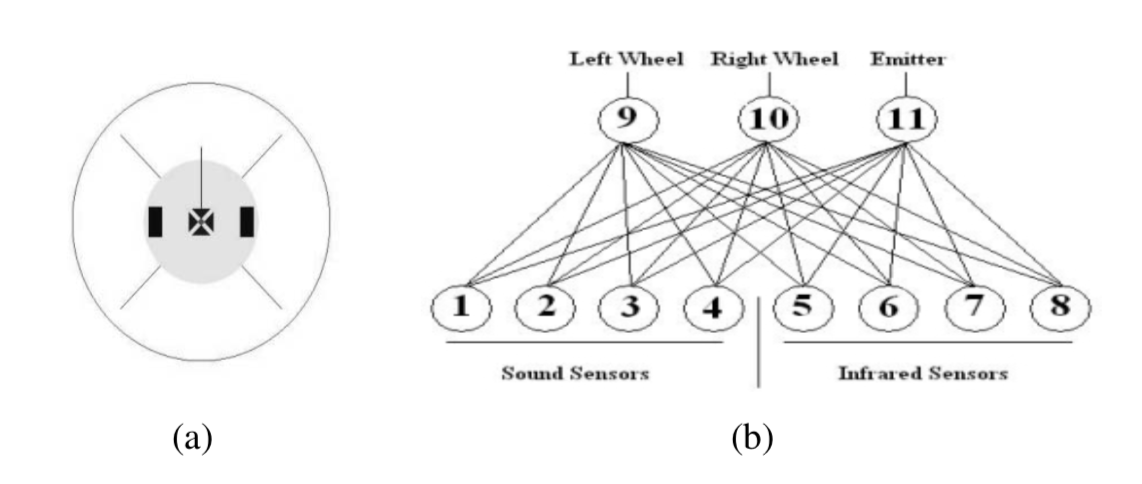
\includegraphics[scale=0.5]{../img/Cobot.png}
\caption{Cobot2D - nákres robota, zdroj : \citep{yalcin2008evolving} }
\end{figure}
\textbf{Fitness funkce}: První použitá $fitness_1$ z tohoto experimentu je obrácená hodnota průměrné vzdálenosti do středu robotické skupiny. 
\par
\begin{center}
\textbf{$fitness_1 = 1/(1/n\sum\limits_{r=1}^{n} d_{rc}) $},
\end{center}
\par 
Kde $n$ je počet robotů v robotické skupině, $r$ je robotův index, $d_{rc}$ je euklidovská vzdálenost mezi $r$ a středem robotické skupiny $c$. 
\par
Druhá $fitness_2$ používá metodu \textit{inverse of hierarchical social entropy} \citep{balch2000hierarchic}. Tato metoda počítá kompaktnost skupiny, tím že hledá každou možnou skupinku (cluster) pomocí změn maximální vzdálenosti $h$ mezi jedinci ze stejného clusteru. Přidávají ještě rozšíření od \textit{Shannon's information entropy}, jenž používá pevné $h$. Toto rozšíření je definováno: 
\par 
\begin{center}
\textbf{$H(h)=-\sum\limits_{k=1}^{M} p_k log_2(p_k)$},
\end{center}
\par 
kde H se nazývá entropie, $p_k$ je proporce jedince z clusteru $k$, $M$ je počet clusterů pro dané $h$. Konečně celý předpis daný Balchem vypadá následovně: 
\par
\begin{center}
\textbf{$fitness_2 = \int_{0}^{\infty} \frac{1}{H(h)dh}$}.
\end{center}
\par 
Použití neuronových sítí a genetického algoritmu se ve výsledku ukázalo jako vhodný prostředek pro učení robotického hejna, neboť se vygenerované chování obstojně shlukuje do úzkých skupin. Autoři dále definují další tzv. cost funkci pro měření úspěchu nalezených chování, aby mohli porovnávat funkce fitness. A $fitness_2$ se ukazuje jako účinější. 
\subsection*{Evoluční strategie a neuronová síť}
V článku \textit{Self-organised path formation in a swarm of robots} \citep{sperati2011self} aplikují pro řízení robotických hejn evoluční strategie. Jako cíl si článek klade problém průzkumu a navigace v neznámém prostředí v kontextu robotických hejn. Experiment, který měl otestovat uvedené vlastnosti robotického hejna, spočíval v co nejrychlejším přesunu celého hejna mezi dvěma prostory v neznámém prostředí. 
\par 
Pro simulaci bylo využito upravené verze OS Evorobota a jako model jedince z hejna e-puck robot \citep{mondada2009puck}. Tento robot se pohybuje pomocí dvou-koleček, má 8 infračervených senzorů, navíc jeden infračervený senzor na povrch a jeden rozpoznávající barvy vpředu (v tomto případě černobílé prostředí). Navíc mu byla přidělána LED vpředu s modrou barvou a červenou vzadu, která může zapínat a vypínat dle potřeby, a také má snímač barev na vrchu. 
\par
Pro ovládání robota zvolili autoři neuronovou síť se 13 vstupy (8 pro infračervené senzory, 1 pro binární podlahový senzor (bílá vs. černá), 4 pro binární vizuální snímače), dále 3 pro skryté neurony a 4 výstupní neurony (2 ovládající kolečka, 2 aktivující přední a zadní led). Formou jsou podobné předchozím modelům robotů. 
\par
Fitness funkce je vyhodnocena po nasazení do robotů a provedení simulace, vlastní fitness je pak průměr z 15 běhů. Ve vyznačených místech se roboti nabíjí, což trvá daný čas a roboti s lepší efektivitou přesunů z jednoho místa do druhého stihnout cestu tam a zpět mnohem rychleji.
\par 
Výsledky prokazatelně ukazují úspěšné použití evolučních strategií na optimalizaci chování robotického hejna. Pro většinu prostředí dokázali najít efektivní řešení.



%%% Fiktivní kapitola s ukázkami tabulek, obrázků a kódu

\chapter{Simulátor}
TODO: Pár stránek o simulátoru
%%% Kapitoly
\chapter{Experimenty}
\section{Úvod}
Všechny práce zmíněné v úvodní kapitole, sice používají evolučních algoritmů k vytvoření řízení chování homogenního robotického hejna, tzn. s pouze jedním druhem robotů. Cílem této práce je najít použití evolučních algoritmů i pro heterogenní hejna. Následující části mají přiblížit obecný postup při hledání optimálního chování hejn, stručně popsat jednotlivé experimenty a poté podrobněji rozebereme každý  experiment zvlášť.
\par 
\subsection{Experimenty}
Pro testování jsem zvolil tři rozličné scénáře. Hlavní motivací bylo jednotlivé úkoly pro hejno udělat komplexnější, aby každá skupina robotů byla schopna řešit pouze část ze zadání scénáře. Také jsem se snažil, aby se scénáře blížily reálným situacím z reálného světa.\par 
\textbf{Pracovní názvy}
\begin{enumerate}
	\item Wood Scene
	\item Mineral Scene
	\item Competitive Scece
\end{enumerate}
\subsubsection{Wood Scene}
Tento scénář je analogií pro kácení lesa, kdy se roboti snaží maximalizovat množství zpracované dřevo na předem vyznačené ploše. První robot plní úkol objevování a kácení stromu, ale neumí je převážet, v mém frameworku se nazývá Wood Scout. Oproti tomu druhý robot má vlastní kontejner na objekty, také je umí zvedat a následně pokládat. Ve frameworku pojmenovaný Wood Worker. Ovšem neumí stromy zpracovávat. Jedná se tedy o úkol typu najdi označ a převez.

\subsubsection{Mineral Scene}
Jedná se o scénář reprezentující sběr surovin pro výrobu paliva a jeho následné využití. Figurují zde 3 rozliční roboti, všichni potřebují pro pohyb  dané množství paliva. Úspěšnost daného hejna se měří množstvím paliva. Nejmenší robot(Mineral scout) disponuje pouze senzory k exploraci prostředí a rádiovým vysílačem pro komunikaci se skupinou. Robot prostřední velikosti(Mineral Worker) se pohybuje o něco pomaleji než Mineral Scout, ale umí přesouvat objekty i více najednou. Robot pro přeměnu minerálu(,suroviny na výrobu paliva,) označen ve frameworku jako Mineral Refactor se přemisťuje nejpomaleji, má možnost přeměnit minerál na palivo. Tento scénář si bere jako inspiraci strategické hry a hypotetické přežití robotů na cizí planetě, kde si budou muset obstarat vlastní 
nerostné suroviny pro běh.

\subsubsection{Competitive Scene}
Poslední ze scénářů se týká soutěže dvou týmů(hejn) ve kterých figurují jeden malý průzkumný robot(Competitive Scout) a jeden vetší bojový robot(Competitive Fighter). Úspěšnost týmu je dána zachovanými jednotkami zdraví robotů a uděleným poškozením do nepřátelské skupiny robotů. Competitive Scout se pohybuje značně rychleji než Competitive Fighter, ale uděluje menší poškození. Což lze opět vztáhnout na chování rozdílných skupin nepřátel např. ve strategických hrách, kde se jejich chování adaptuje, co nejlépe na dané prostředí. 
\subsection{První Kroky}
\unsure{Pravděpodobně špatný název kapitoly}
\par
Nejvíce se budu věnovat prvnímu scénáři, protože jsem na něm strávil většinu času a testoval na něm různé postupy. Také jsem jej používal  jako benchmark pro počítání průsečíků, paralelního zpracování jednotlivých generací, v neposlední řadě sloužil pro odhalení většiny chyb simulace, návrhu vizualizace a formátu souboru pro nastavení ES,DE. Nakonec se ukázalo, že postup aplikovaný na jeho řešení je rentabilní i pro další dva scénáře. Takže pro další dva scénáře už bylo klíčové nalézt pouze fitness funkci a nastavení parametrů DS a ES.
\par
V úvodu bych se také rád zmínil o prvotních pokusech řešení problému evoluce heterogenní skupiny robotů právě na prvním ze scénářů. Nejdříve jsem pro otestování prostředí a ověření dostatečné obtížnosti testovacích scénářů zkoušel generovat náhodné neuronové sítě a po-té měřit jejich úspěšnost. Pokud jsem se soustředil pouze na hlavní úkol a roboti nebyly hodnoceny za žádné další interakce, tak žádný ani z 20 000 jedinců nedosáhl na jiné hodnocení než 0. Což prokázalo komplexnost scénářů a jich obtížnost.
\par 
Dále nastal čas vyzkoušet evoluční algoritmy pro vytvoření chování(, tzn. optimalizaci neuronové sítě). Zvolil jsem, stejně jako v předchozím případě, fitness funkci hodnotící pouze hlavní cíl scénáře. Tento postup se také ukázal opět jako nedostatečný, jelikož žádná z náhodně vytvořených neuronových sítí nebyla schopna řešit žádným způsobem (, ani velmi hloupě). Diferenciální evoluce se v tomto případě chovala velmi podobně jako "random search" algoritmus, jelikož hodnota fitness byla pro  všechny řešení 0,. Evoluční strategie měly problém se pohnout jakýmkoli směrem, protože směr prohledávání řešení je závislý na velikostech fitness. Což lze jednoduše vypozorovat z definice algoritmu v kapitole \ref{sec:ES} o ES. Takže i tento postup se ukázal bez jakéhokoli výsledku. \unsure{Nenapadá mě, jak kreslit graf s nulovou fitness, nakreslit vzdálenosti mezi jednotlivými neuronkami?}
\redo{Přidat tabulku s parametry funkce těchto běhů} 
\par 
Dalším vylepšením bylo přidat některé meta-úkoly, které budou jednoduché a dosažitelné i pro vygenerované algoritmy. Předpokládal jsem, že jejich postupné vylepšování evolučními algoritmy povede k řešení složitějších úkolů a nakonec až k hlavnímu cíli. Například zahrnout fitness počet navštívený částí mapy, už před připraveným objektů a podobně. V ideální případě by se měla populace blížit k ideálnímu řešení jednoho z jednodušších meta-úloh. Díky tomu by mělo být jednoduší narazit na chování řešící i složitější úlohy, protože spolu evidentně souvisí. Což můžeme ilustrovat na WoodScene scénáři, kde roboti prozkoumávající rychle a ve velké rozptylu mají možnost pokácet vícero stromů. I přes mé optimistické výhledy se ukázalo, že jedinci jsou díky složitější fitness funkci mnohem náchylnější k zaseknutí v lokálním optimu. Zasekávaly se u jednodušších úkolů, vylepšovali jen je. Nové komplexnější chování se objevilo velmi zřídka a jedinci obdařeny těmito vlastnosti opět vylepšovali pouze jednoduché chování. Pokusil jsem se zabránit zaseknutím v lokálních maximech přes různé ohodnocení fitness, ale výsledky opět neukázali přívětivé.\par
Z předchozích zkušeností jsem usoudil, že bude potřeba vytvořit nějakou postupnou cestu k řešení tolik náročného cíle. \unsure{Můžu přiznat, že mi vedoucí radí?} Na základě konzultací se svým vedoucím jsem vytvořil koncept meta-úkolů, jedná se o jednodušší úlohy vedoucí k té hlavní. Od předchozího postupu se odlišuje oddělením jednotlivých fitness funkcí odpovídající meta-úkolu. Použiji evoluční algoritmy s fitness funkcí pouze aktuálního meta-úkolu a po dosažení dostatečné úrovně splnění meta-úkolu, vezmu vytvořenou generaci a použiji na ní evoluční algoritmus s fitness soustředěnou na následující meta-úkol. Tento postup opakuji až jako fitness funkci použiji vlastní ohodnocení scénáře. Uvedený přístup konečně vedl k uspokojivým výsledkům a jednotlivé průběhy budou popsány v dalších kapitolách. 
\section{Použité algoritmy}
\redo{Předělat tuto kapitolu}
Vybral jsem dva evoluční algoritmy, které se zdáli při prvotních testech nejvíce perspektivní. Při evoluci homogenních robotů se nejčastěji používají Evoluční Strategie jako jeden z optimalizačních algoritmů, také proto jsem je zvolil jako jeden z využívaných algoritmů. Druhá volba padla na o něco méně agresivní optimalizaci v podobě Diferenciální Evoluce. Oba algoritmy jsou popsány v kapitole o evolučních algoritmech. \par 
Při prvotních zkušebních optimalizací se ukázalo, že optimalizovat rovnou celý cíl jednotlivých scénářů není příliš slibné. Po konzultaci s vedoucím, jsem se rozhodl rozdělit vždy cíl na jednotlivé pod-úkoly hlavního cíle scénáře. Jednotlivé pod-úkoly neřeší vždy všichni roboti najednou, ale některé jen homogenní skupina. Nicméně nejpozději v posledním pod-úkolu už jsou evolvovány společně.
\par
Zkoušel jsem také testovat, roboty s paměťovými sloty oproti těm bez. Úspěšnost a konvergence robotů s pamětí se znatelně se učil pomaleji. Roboty bez slotů se nebyly schopni přiblížit k výsledkům těm s pamětí ani při velkém počtu generací. Z tohoto důvodu všichni roboti mají připojeno alespoň 10 paměťových slotů. Paměťový slot zároveň chová jako senzor i jako efektor. 
\par 
Jako samozřejmostí u každého robota najdeme line senzory, touch senzory, dvou-kolečkový motor, lokátor. \par 

\subsection{Diferenciální Evoluce}
 \redo{Nastavení parametrů, varianta, praktická implementace}

\subsection{Evoluční strategie}
\redo{Nastavení parametrů, varianta, praktická implementace}


\section{WoodScene experiment}
Cílem tohoto scénáře je shromáždit uprostřed mapy, co nejvíce zpracovaného dřeva. Plocha pro skládání dřeva je označena rádiovým signálem s hodnotou signálu 2. V experimentu se dohromady celkem vyskytuje 9 robotů dvou různých druhů. Roboti jsou na začátku simulace umístěni uprostřed mapy na skládacím prostoru, po-té následuje 2000 iterací simulace mapy. 

\subsection{Roboti}

\subsubsection{Scout robot}
Jedná se o robota, který má na starosti průzkum mapy a kácení nalezených stromů. Pro komunikaci s ostatními roboty má možnost vysílat rádiový signál s hodnotou 0. Oproti Worker robotovi je menší, rychlejší, jeho senzory mají větší dosah, navíc proti němu disponuje type senzorem a refaktorem nalezených stromů. Type senzor představuje formu radaru, říká robotovi s jakou četností se vyskytují v dosahu senzoru. Refaktor reprezentuje techniku kácení mění strom na dřevo. 
\par 
\begin{center}
\begin{tabular}{l  l  l l @{\hspace{1.5cm}}D{.}{,}{3.2}D{.}{,}{1.2}D{.}{,}{2.3}}
        \toprule
        Tvar: & Kruh & Poloměr: & 2.5 \\
        Název: & WoodCutterM \\
        Velikost kontejner: & 0 \\
        \hline
        Efektory \\
        \midrule
        Motor: & Dvou kolečkový & Maximální rychlost: & 3 \\
        Kód rádiového signálu: & 0 & Poloměr signálu: & 200\\
        Refaktor: & $Strom \Rightarrow Dřevo$ & Dosah refaktoru: & 10\\
        Počet paměťových slotů: &10 & Obsah slotu: & float\\
        \hline 
        Senzory \\
        \midrule
        Počet line senzorů: &  3 & délka: & 50\\
        Orientace line sensorů: & $0^\circ$ & $45^\circ$ & $-45^\circ$\\
        Type senzor: & Poloměr: & 50\\
        Rádiový přijímač: & Poloměr: & 100 \\
        Touch senzory: & Počet: & 8 \\  
        Lokátor senzor\\ 
        \bottomrule
\end{tabular}
\end{center}
\subsubsection{Worker robot}
Worker robot se stará o transport objektů na mapě. Ke komunikaci využívá signálů s kódem 1. Sebrané objekty ukládá do kontejneru, kam se vejde 5 entit. Zvedání a pokládání probíhá skrze efektor Picker. 
\par 
\begin{center}
\begin{tabular}{l  l  l l @{\hspace{1.5cm}}D{.}{,}{3.2}D{.}{,}{1.2}D{.}{,}{2.3}}
                \toprule
                Tvar: & Kruh & Poloměr: & 5\\
                Název: & WoodWorkerM \\
                Velikost kontejner: & 5\\
                \hline
                Efektory \\
                \midrule
                Motor: & Dvou kolečkový & Maximální rychlost: & 2 \\
                Kód rádiového signálu: & 0 & Poloměr signálu: & 200\\
                Picker: & Dosah pickeru: & 10\\
                Počet paměťových slotů: &10 & Obsah slotu: & float\\
                \hline 
                Senzory \\
                \midrule
                Počet line senzorů: &  3 & délka: & 30\\
                Orientace line sensorů: & $0^\circ$ & $45^\circ$ & $-45^\circ$\\
                Rádiový přijímač: & Poloměr: & 100 \\
                Touch senzory: & Počet: & 8 \\  
                Lokátorový senzor\\ 
                \bottomrule
\end{tabular}
\end{center}

\subsection{Vyhodnocování Fitness}
Fitness funkce pro ohodnocení WoodScene scénáře probíhá vždy až na konci simulace. I když se úspěšnost v pod-úkolech  vždy posuzuje jinak, celou fitness funkci lze shrnout do následujícího cílů. Roboti jsou odměňováni za: 
\begin{enumerate}
        \item kolize = počet pokusů o pohyb při kterém by došlo ke kolizi 
        \item nalezené stromy = stromy o které zavadil line senzor 
        \item pokácené stromy = stromy, které refaktor změnil 
        \item sebrané dřevo = zpracované dřevo, které mají roboti uvnitř kontejnerů 
        \item uskladněné dřevo = dřevo, které dovezli na vyznačené místo 
\end{enumerate}

\subsection{Pod-úkoly} 
Pro oba použité algoritmy jsem používal stejné úlohy pro naučení robotů postupně těžších a těžších cílů. Hlavně také, abych mohl porovnat oba evoluční algoritmy. \redo{Bojím se, že pro ES to nebude stačit} 
\begin{enumerate}
        \item vygenerování robotů = Na začátku je vygenerováno chování robotů naprosto náhodně. Pro každého robota, je vygenerována náhodná jednovrstvá neuronová síť. 
        \item učení chůze = Pro oba roboty je velmi důležité, aby se pohybovali bez kolizí po celé mapě a objevovali, co největší prostor. Roboti jsou vyvíjeni odděleně a fitness se soustředí na počet kolizí(záporným ohodnocením) a na nalezené stromy(kladným ohodnocením).
        \item těžba stromů = Scout roboty, kteří se už obstojně po mapě pohybují, je třeba naučit kácet stromy. Proto dalším pod-úkol cílí ve fitness funkci na počet pokácených stromů. Nicméně stále také na počet stromů nalezených. 
        \item převoz dřeva = Správně pohybující chceme naučit sbírat vytěžené dřevo. Fitness hodnotí počet sebraného dřeva, případně i uskladněné dřevo. Na těchto mapách jsou už na začátku připraveny pouze entity zpracovaného dřeva.
        \item kooperace = V posledním experimentu, se hodnotí pouze sebrané a uskladněné dřevo. A evolvují se oba druhy robotů současně. 
\end{enumerate}

\subsection{Nastavení EA}
\subsubsection{Diferenciální Evoluce}
Pro diferenciální evoluci jsem zvolil 100 jedinců jako velikost populace, kteří procházejí přes 1000 generací. Mezi nejtěžší přípravy evolučních algoritmů patří volba parametrů evoluce u DE se konkrétně jedná o pravděpodobnost křížení(CR) a váhu diference(F) (, v angličtině se nazývá Differential weight). Po první testech jsem uvážil $F = 0.8 $ a $CR = 0.5$ jako nejlepší volbu. 
\subsubsection{Evoluční Strategie}
U Evolučních Strategiích, které mají trochu jinou formu mutací, budu evolvovat 8 jedinců. Tyto jedinci projdou 200 generací a velikost mutačního kroku  v každé generaci je právě 20. Varianta $(\sigma,\lambda)$ se ukázala jako vhodnější volba, neaplikuji tedy elitismus, při testech se stávalo, že se jedinec na začátku zasekl v lokálním optimu a dál se vůbec nevyvíjel. Jako learning rate neboli alpha se osvědčila hodnota 0.05 a rozptyl u šumů normálního rozdělení sigma roven 0.1.
\subsection{Výsledky Experimentu}
\subsection{První běh}
Pro ověření správnosti obou evolučních algoritmů jsem nejprve, v mém programu sloužícímu k optimalizaci, pozoroval chování robotů s náhodně vygenerovaným chováním, kdy se většina z nich točila dokola uprostřed mapy a objevila pouze objekty v nejbližším okolí. Oba druhy robotů použité v WoodScene scénáři se od sebe v podstatě v chování nelišily. První pod-úkol, který měl naučit pohybu, jak WoodWorker robota tak WoodCutter robota, jsem nastavil dle následujících tabulek. WoodWorker je ohodnocen za nález zpracovaného dřeva a WoodCutter za stromů, aby se připravovali na budoucí hlavní úkol.\par
\redo{Tabulka s konkrétním nastavením fitness \textbf{WoodCutter} pro první úlohu.} \par
\redo{Tabulka s konkrétním nastavením fitness \textbf{WoodWorker} pro první úlohu.} \par
\par
Po dokončení evoluce prvního pod-úkolu, se v populaci už dále neobjevovali jedinci, kteří by měli problém s pohybem. Vyhýbali se překážkám a snažili se rozptýlit po, co největší ploše. Nejlepší z jedincí byli schopni objevit až 80\% všech stromů na mapě. Na následujících dvou grafech můžeme pozorovat změnu hodnotu fitness u každého EA a druhu robota. Co se týče porovnání WoodWorkera a WoodCuttera, tak si WoodCuttera vedl znatelně lépe, což přisuzuji větší délce jeho line senzorům a absenci type senzoru u WoodWorkera. Tento pod-úkol by se dal považovat za benchmark obou optimalizačních algoritmů a také za kontrolu jejich správnosti. 



\chapter*{Závěr}
\addcontentsline{toc}{chapter}{Závěr}
V rámci této práce byl implementován kompletní 2D simulátor umožňující simulovat chování robotických hejn, simulátor umožňuje hejnu, abys se skládalo z rozličných jedinců. Tento simulátor také obsahuje metody EA, konkrétně DE a ES jako prostředky pro optimalizaci řízení robotických hejn. Pro vizualizaci těchto chování vznikl program umožňující prohlížení už optimalizovaných chování. Simulace byla také optimalizována a bylo použito paralelního zpracování. 
\par
Za pomocí těchto programů byla otestováno evolucí generované ovládání heterogenních hejn v rámci tří rozličných scénářů. Úkoly v těchto scénářích byly tvořeny z tradičních problémů robotických hejn jako je shlukování, pohyb v prostředí, rozptylování, apod. Dohromady tvořily scénáře komplexní problémy s netriviálním řešením. 
\par
Během prvního experimentu byly porovnány dva evoluční algoritmy pro optimalizaci neuronových sítí pro řízení heterogenních  swarmů, konkrétně se jednalo o DE a ES. V rámci toho experimentu bylo provedeno několik testovacích běhů pro zmíněné srovnání. DE se ukázala jako lepší varianta pro optimalizaci heterogenního robotického hejna. 
\par 
V dalších dvou experimentech se bylo potvrzeno, že tuto metodu lze použít jako vhodný nástroj pro optimalizaci jednoduchých chování hejna. Ovšem objevily se i limity spojené s obtížnými úkony, kde DE nepracovala uspokojivě. Bylo navrženo řešení těchto nedostatků, ovšem z časových důvodů nebylo vyzkoušeno. 

\subsection*{Možná rozšíření}
Tato práce poskytuje řadu zajímavých možností k rozšíření ať už se jedná o řešení nevyzkoušených metod na neúspěšných scénářích či porovnání s jinými metodami.\par
V rámci nedostatků scénářů Mineral Scene a Competitive Scene by bylo žádoucí vyzkoušet evoluční algoritmy, které umí generovat složitější neuronové sítě. Jedná se především o algoritmy odvozené z NEAT rodiny. Otestovat je na těchto obtížných scénářích.
\par
Pro porovnání úspěšnosti evolučního algoritmu s jinýmu učícími algoritmy by bylo vhodné otestovat DE a ES s tradičním \textit{backpropagation} algoritmem pro neuronové sítě. 
\par
V neposlední řadě by zajímavou cestu tvořilo přenesení vyvinutých chování na fyzické roboty. Což by ale vyžadovalo velké úpravy na simulátoru, protože simulátor značně zjednodušuje akce v prostředí. Navíc by bylo třeba přidat šumy prostředí neboť senzory jsou jimi v reálném světě značně zkresleny. 

%%% Seznam použité literatury
%%% Seznam použité literatury (bibliografie)
%%%
%%% Pro vytváření bibliografie používáme bibTeX. Ten zpracovává
%%% citace v textu (např. makro \cite{...}) a vyhledává k nim literaturu
%%% v souboru literatura.bib.
%%%
%%% Příkaz \bibliographystyle určuje, jakým stylem budou citovány odkazy
%%% v textu. V závorce je název zvoleného souboru .bst. Styly plainnat
%%% a unsrt jsou standardní součástí latexových distribucí. Styl czplainnat
%%% je dodáván s touto šablonou a bibTeX ho hledá v aktuálním adresáři.

\bibliographystyle{czplainnat}    %% Autor (rok) s českými spojkami
% \bibliographystyle{plainnat}    %% Autor (rok) s anglickými spojkami
% \bibliographystyle{unsrt}       %% [číslo]

\renewcommand{\bibname}{Seznam použité literatury}

%%% Vytvoření seznamu literatury. Pozor, pokud jste necitovali ani jednu
%%% položku, seznam se automaticky vynechá.

\bibliography{literatura}

%%% Kdybyste chtěli bibliografii vytvářet ručně (bez bibTeXu), lze to udělat
%%% následovně. V takovém případě se řiďte normou ISO 690 a zvyklostmi v oboru.

% \begin{thebibliography}{99}
%
% \bibitem{lamport94}
%   {\sc Lamport,} Leslie.
%   \emph{\LaTeX: A Document Preparation System}.
%   2. vydání.
%   Massachusetts: Addison Wesley, 1994.
%   ISBN 0-201-52983-1.
%
% \end{thebibliography}


%%% Obrázky v bakalářské práci
%%% (pokud jich je malé množství, obvykle není třeba seznam uvádět)
\listoffigures

%%% Tabulky v bakalářské práci (opět nemusí být nutné uvádět)
%%% U matematických prací může být lepší přemístit seznam tabulek na začátek práce.
\listoftables

%%% Použité zkratky v bakalářské práci (opět nemusí být nutné uvádět)
%%% U matematických prací může být lepší přemístit seznam zkratek na začátek práce.
\chapwithtoc{Seznam použitých zkratek}

%%% Přílohy k bakalářské práci, existují-li. Každá příloha musí být alespoň jednou
%%% odkazována z vlastního textu práce. Přílohy se číslují.
%%%
%%% Do tištěné verze se spíše hodí přílohy, které lze číst a prohlížet (dodatečné
%%% tabulky a grafy, různé textové doplňky, ukázky výstupů z počítačových programů,
%%% apod.). Do elektronické verze se hodí přílohy, které budou spíše používány
%%% v elektronické podobě než čteny (zdrojové kódy programů, datové soubory,
%%% interaktivní grafy apod.). Elektronické přílohy se nahrávají do SISu a lze
%%% je také do práce vložit na CD/DVD. Povolené formáty souborů specifikuje
%%% opatření rektora č. 23/2016.
\chapwithtoc{Přílohy}

\openright
\end{document}
